\section{Evaluation}
\label{sec:evaluation}

We evaluate the performance of our solution on a single Amazon EC2 c4.xlarge instance, running Debian 8.3 (Jessie) and equipped with an Intel Xeon E5-2666 Haswell (2.6 GHz, 4 cores and 25 MB cache), 8 GB of RAM and SSD with 900 IOPS~\cite{AWSEC2InstanceTypes}. This experimental environment is very similar to that employed for evaluating the Grand Challenge solutions~\cite{GrandChallenge:2016}. 
%
Our solution is implemented in Java 1.8 and relies on Apache Flink 1.0.0~\cite{Flink} and Redis 3.0.7~\cite{Redis}.

The experimental analysis evaluates for both queries 
(1) the latency distribution on crucial operators, 
(2) the average latency per tuple,  
and (3) the average memory utilization.
%
The latency is measured using the analysis tools provided by the Flink framework, whereas the memory utilization is recorded every second during the application execution.

Our solution aims at properly processing the dataset proposed by the Grand Challenge in a timely way. This dataset presents $ 55.9 \times 10^6 $ events, distributed as: $ 44 \% $ comments, $ 39\% $ likes, $ 15\% $ posts, and $ 2\% $ friendships.
%
Preserving this event distribution, our experimental evaluation considers portions of the dataset ranging from $ 1\% $ ($ 55.9 \times 10^3 $ events) to $ 50\% $ ($ 27.9 \times 10^6 $ events) of the original dataset.
%
We parametrized the second query to identify the top-$3$ comments supported by the larger communities with a sliding window of 1 hour (i.e., $k = 3 $, $d = 3600 $~s).

To inspect the latency distribution, we can partition the topology into the following meta-operators: 
\begin{enumerate} \itemsep0em
	%
	\item \textit{Src-Snk:} 
	which encapsulates the logic involved in introducing and producing the events. It comprises latencies due to the I/O operations and the generation of tuples that allows to compute the scores (i.e., event ordering, time synchronization, comment to post mapping);
	%
	\item \textit{Updater:} 
	which encapsulates the logic involved in computing the post or comment score. It comprises the most memory-intensive data structures, the feedback stream (first query), and clique computation (second query).
	%
	\item \textit{Ranker:} 
	which encapsulates the logic involved in ranking the posts/comments and filtering the updates. It comprises latencies due to the step-wise sorting and ranking approach. 
	%
\end{enumerate}

During all the experiments, approximately half of the latency is introduced by the \textit{Updater} and about a third by the \textit{Ranker}.

\begin{figure}
	\centering
	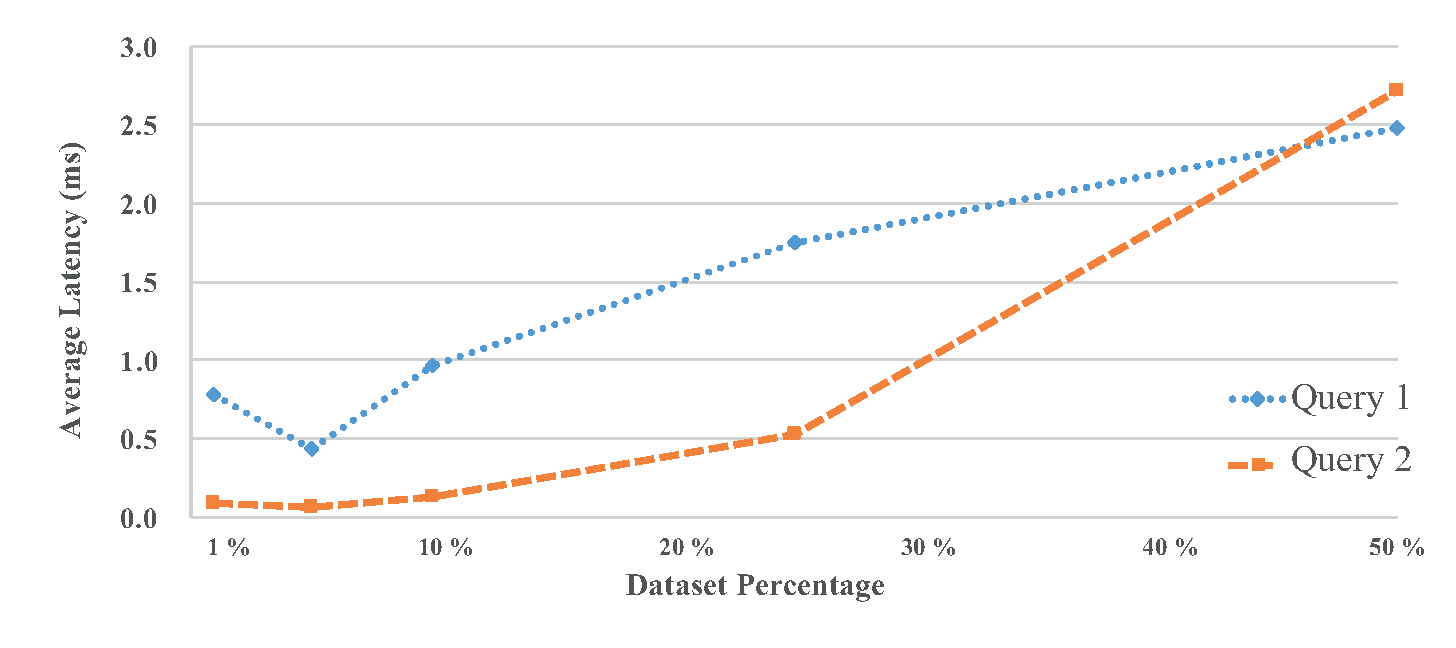
\includegraphics[width=\columnwidth]{fig/latency_prop_final2}
	\caption{Query 1 and Query 2: average latency per tuple.}
	\label{fig:latency}
\end{figure}

\begin{figure}
	\centering
	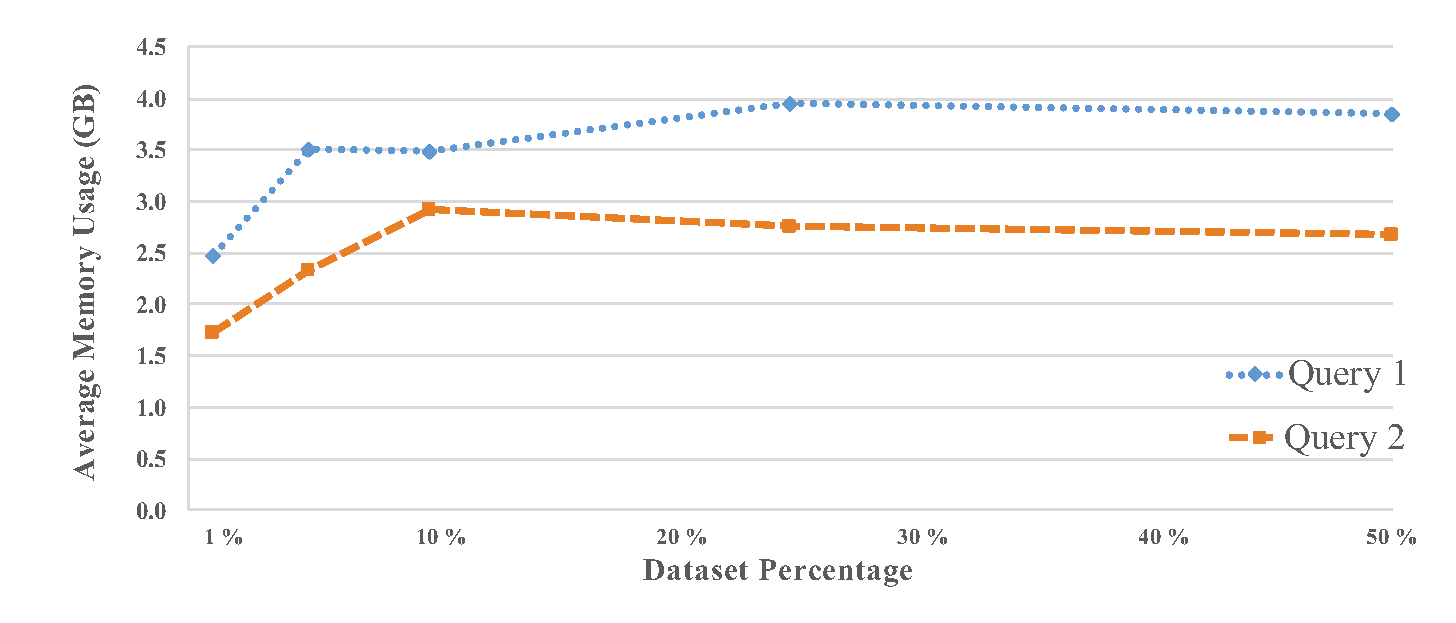
\includegraphics[width=\columnwidth]{fig/memory_prop_final}
	\caption{Query 1 and Query 2: average memory utilization.}
	\label{fig:memory}
\end{figure}

The average latency per tuple of both queries is represented in Figure~\ref{fig:latency}.
%
As the dataset increases in size, the trend of this metric becomes clearer.
%
For the first query, the average latency increases almost linearly with the dataset size; this trend is due to the growing number of post scores that the system has to manage. 
%
For the second query, the average latency increases exponentially as the dataset grows, and, upto the $ 30 \% $ of the dataset, the system achieves latencies lower than $ 1 $~ms. 
The performance trend of this query is readily explained recalling that (1) the application has to maintain in memory the whole social-graph, and (2) identifying the cliques is an NP-hard problem. 
Moreover, we have obtained empirical evidences that the centralized usage of Redis for small and high-frequency updates shows poor performances. 

As regards the memory utilization, Figure~\ref{fig:memory} shows a comparison of this metric for both the queries.The general tendency shows that the required memory reaches a steady state below $ 4 $~GB.
%
In the first query, this result is achieved thanks to the feedback stream which allows to discard all the data (e.g., comments, score) concerning the expired posts. 
%
Observe that the advantage of exploiting the feedback stream is proportional to the amount of posts and to their expiration rate.
%
In the second query, the memory utilization stabilizes around $ 3 $~GB when the application processes at least $ 10 \% $ of the whole dataset.
Evaluating the memory utilization trend, we can suppose that most of the social graph structure is built quickly while it tends to evolve slowly. 
%
When the dataset grows over the $ 25 \% $, an increasing computational effort is due to the management of Redis, slowing down the task of identifying the largest communities. 

Summing up, the experimental results show that our solution provides  \textit{effective load balancing} because the workload is balanced among the operators and cores, thus making our solution not affected by back-pressure phenomena in any portion of the stream and in any stage of computation;
there is also an \textit{efficient memory usage}, because the physical memory is never close to saturation, thus avoiding the overhead introduced by the garbage collection and memory swapping. 
However, there are some \textit{latency bottlenecks} that slow down the application execution, mainly due to the presence of centralized and complex operators. 
